\chapter{Der Kobold Client}
Der Client basiert grundlegend auf der Eclipse Plattform und deren Widgettoolkit und ist
dadurch von dessen nativer Schnittstelle abh�ngig. Laut dem Eclipse Consortium werden die folgenden 
Plattformen und Betriebssysteme unterst�tzt:
\begin{itemize}
    \item Windows NT/2000/XP
    \item Linux (x86/Motif)
    \item Linux (x86/GTK 2)
    \item Solaris 8 (SPARC/Motif)
    \item QNX (x86/Photon)
    \item AIX (PPC/Motif) 
    \item HP-UX (HP9000/Motif)
    \item Mac OSX (Mac/Carbon)
\end{itemize}
Er wird als Feature-Set implementiert und mit eigenem Product Branding versehen.
Das Product Branding umfasst die �nderung der Fensternamen und der Produkticons, sowie
einer Willkommensseite die einen kurzen �berblik �ber Funktionalit�t und Zweck des Kobold Tools geben soll.

Das Feature-Set wird als Set von inernationalisierbaren Eclipse Plugins implementiert.
Die Ausgangsperspektive wird aus 4 Teilen bestehen:
\begin{itemize}
	\item Der Produktlinienarchitektur View/Editor
	\item Der Rollen View
	\item Der Worklflow/Task View
	\item Die Minimap
\end{itemize}
Diese werden in den jeweiligen Unterkapiteln n�her beschrieben.
Um das Rollenprinzip konsistent durchzusetzen ist eine zentrale Anmeldung an einem Server n�tig.
Details zu der Serverseitigen L�sung finden sie auf Seite %todo Link zur Serverseite% 
. 
\section{Authentifizierung}
Die Authentifizierung am Server erfolgt durch einen RPC. Der Benutzer kann bei der Erstbenutzung des 
Clients w�hlen ob er sich bei jedem Programmstart authentifiziern soll, oder ob das Passwort
und der Benutzername gespeichert werden sollen.
\section{Der Produktlinienarchitektur View/Editor}
In diesem View wird die je nach aktiver Rolle relevante Sicht auf die Architektur der Produktlinie
angezeigt. Die grafische "Notation" h�lt sich dabei an die in dem Paper ... festgelegte Struktur.
Um dies nocheinmal grafisch darzustellen hier noch einmal die 3 verschiedenen Sichten auf die
Produktlinien bzw. Produktarchitektur.
Die Ansicht bietet die M�glichkeit verschidene Zoomstufen einzustellen. Dies reultiert darin,
dass im aktuellen Ausschnitt m�glicherweise nicht die ganze Architektur zu sehen ist.
Um trotzdem den �berblick zu gew�hrleisten wird eine Minimap zur Verf�gung gestellt.
%todo Grafiken einf�gen%
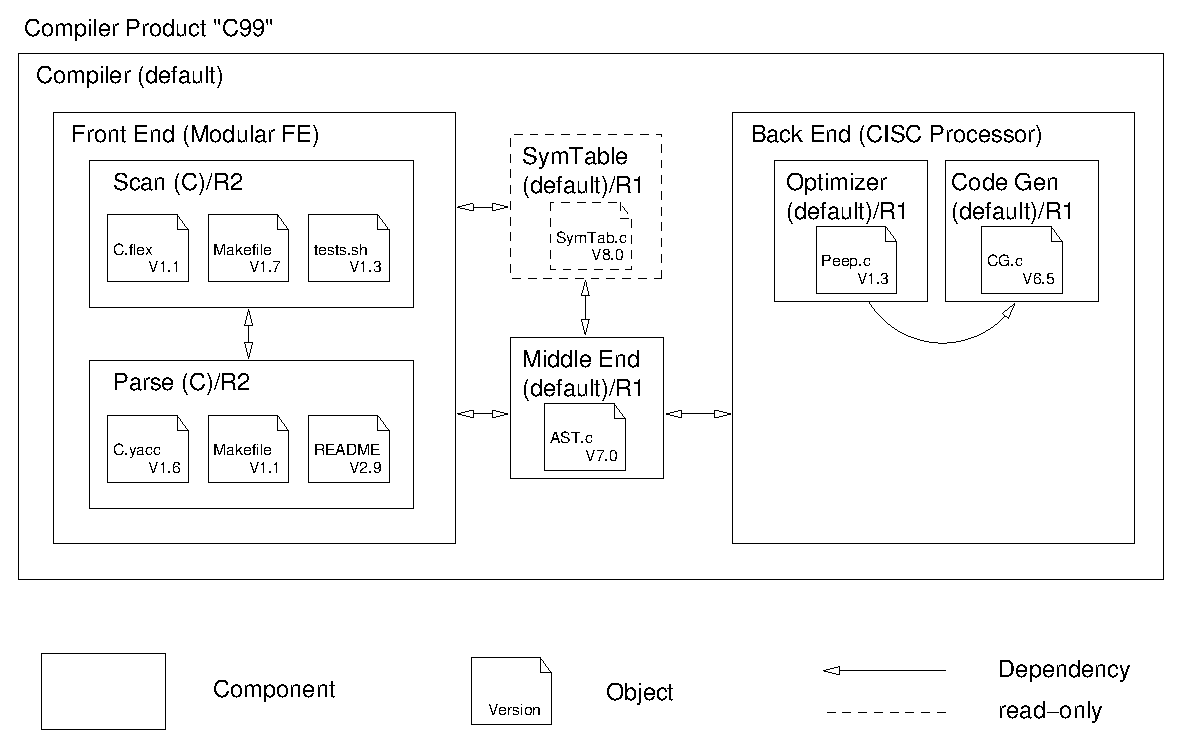
\includegraphics[width=15cm]{compiler-p}
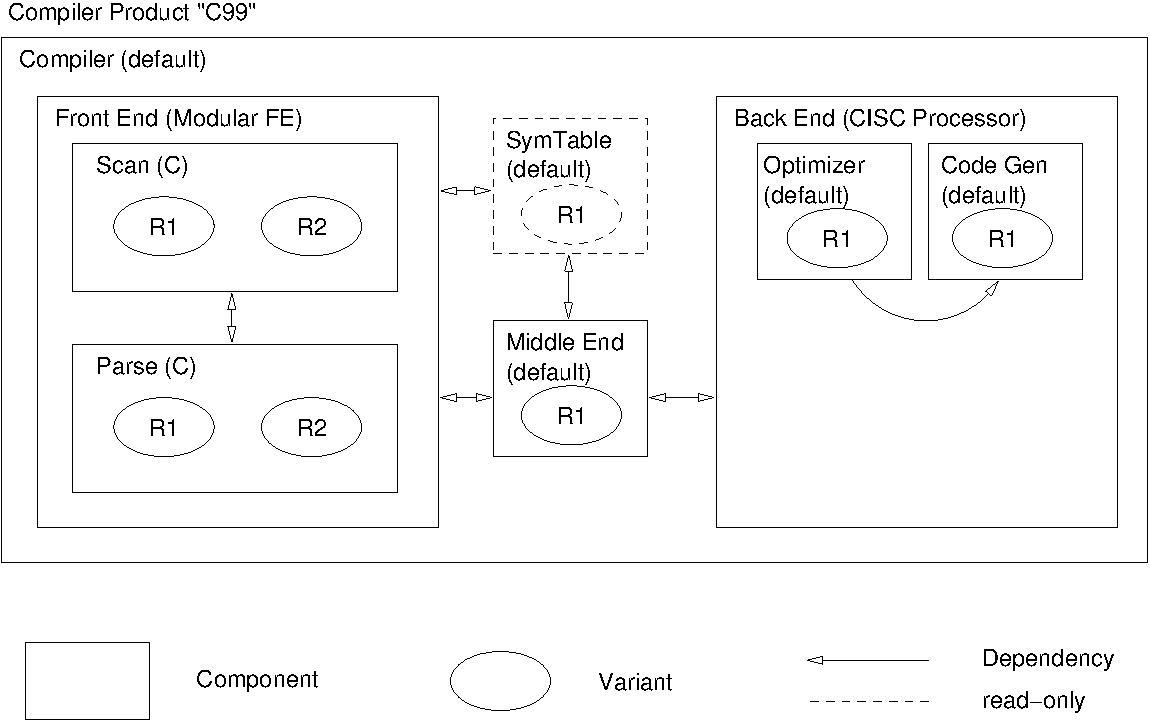
\includegraphics[width=15cm]{compiler-pe}
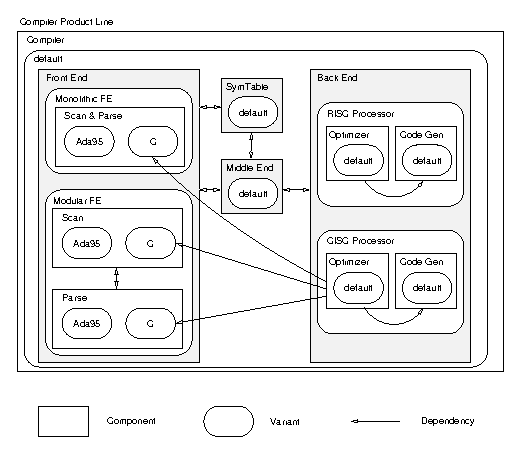
\includegraphics[width=15cm]{compiler-spl}
\section{Der Rollen View}
Auf der linken Seite der Ausgangsperspektive wird ein hierarchischer Baum angezeigt, der
die momentan aktive Rolle und die mit Ihr verbundenen m�glichen Sichten darstellt.
\section{Der Worklflow/Task View}
Am unteren Rand der Ausgangsperspektive wird standardm�ssig 
\section{Die Minimap}
Am rechten unteren Rand der Ausgangsperspektive wird eine sogennante Minimap angezeigt,
in der ein �berblick �ber die ganze Architektursicht der aktuellen Rolle gegeben wird.
